\documentclass[aip, jcp, reprint, onecolumn, nofootinbib]{revtex4-2}

\bibliographystyle{apsrev4-2}

\usepackage{physics}
\usepackage{amsmath}
\usepackage{amssymb}
\usepackage{mathtools}
\usepackage{graphicx}
\usepackage{dcolumn}
\usepackage[colorlinks=true, linkcolor=black, urlcolor=blue, citecolor=black, anchorcolor=black]{hyperref}

%supplementary figs
\renewcommand{\thefigure}{S\arabic{figure}}
\renewcommand{\thetable}{S\arabic{table}}
\renewcommand\theequation{S\arabic{equation}}
\renewcommand*{\thepage}{S\arabic{page}}

\graphicspath{{"figures/"}}
\begin{document}
%Title of paper
\title{Supporting Information for Coherent IR-Hyper-Raman Four Wave Mixing Spectroscopy}


\author{Ryan P. McDonnell} 
\author{Daniel D. Kohler}
\author{John C. Wright} \email{wright@chem.wisc.edu}

\affiliation{Department of Chemistry, 
        University of Wisconsin - Madison, 
        Madison, Wisconsin 53706, 
        United States of America}

\date{\today}

\maketitle
\tableofcontents
\clearpage


\section{Evaluating Herzberg-Teller Integrals for Harmonic Wells of Identical Curvature}

In this section, we discuss the evaluation of Herzberg-Teller integrals when the ground and first excited state are harmonic wells of identical curvature.\cite{HerzbergTeller1933}
% We note that Myers et al. have developed a general expression to evaluate Franck-Condon factors for two displaced harmonic wells of differing curvature,\cite{Myers1982} 
We investigate the one dimensional case using the Hamiltonian described in the main text, $H = H_g |g) \left(g| + H_e |e\right) (e|$, where
\begin{subequations}\label{Hamiltonian}
	\begin{equation}
		H_g = \frac{\hbar \omega }{2} \left(p^2 + q^2 \right)
	\end{equation}
	and
	\begin{equation}
		H_e = \frac{\hbar \omega }{2} \left(p^2 +  (q-\Delta)^2 \right) + \hbar \omega_{eg}.
	\end{equation} 
\end{subequations}
Here, $p,q$ are the dimensionless conjugate normal mode coordinates, $\hbar\omega_{eg}$ is the energy difference between $H_e$ and $H_g$, and $\Delta$ is the dimensionless offset of the excited state surface relative to the ground state.
The Hamiltonians are quantum harmonic oscillators.
The solutions to the harmonic oscillator Hamiltonian are well known, and their position space wavefunctions are
\begin{equation}
	\psi_m(q) = \langle q | m \rangle = N_m H_m(q) \exp(-q^2/2),
\end{equation}
where $N_m = (m! \ 2^m \pi^{\frac{1}{2}})^{-\frac{1}{2}}$ is the normalization factor and $H_m$ is the $m^{th}$ Hermite Polynomial.\cite{RN230, MorseFeshbach}

For an $n$-quantum excited state vibration $| \tilde{n} \rangle$, and a $m$-quantum ground state vibration $\ket{m}$, the $k^{th}$-order vibrational coupling term is
\begin{equation}
	\begin{split}
		\mel{\tilde{n}}{q^k}{m} &= \int_{-\infty}^\infty \mathrm{d}q \ \psi^*_n(q-\Delta) q^k \psi_m(q)\\
		&= \int_{-\infty}^\infty \mathrm{d}q \ N_n H_n(q-\Delta) \exp(-\frac{(q - \Delta)^2}{2}) q^k N_m H_m(q) \exp(-\frac{q^2}{2}). \\
		&= N_n N_m \exp(-\frac{\Delta^2}{2}) \int_{-\infty}^\infty \mathrm{d}q \ H_n(q-\Delta) q^k H_m(q) \exp(-q^2 + q\Delta)
	\end{split}\label{key}
\end{equation}
The integral corresponds to Franck-Condon factors for $k=0$ and Herzberg-Teller matrix elements for $k=1$.
The vibrational coupling integrals are written assuming the expansion of the dipole moment is taken about the equilibirum point of the ground state geometry ($q=0$), as is done in the main text.
Note that in the limit $\Delta \rightarrow 0$, typical harmonic oscillator selection rules are restored, as the two wells have the same vibrational Hamiltonian and thus share an identical subspace of orthonormal eigenstates.

\subsection{General Solution to $\langle \tilde{n} | q^k | m \rangle$}
The matrix elements of \autoref{key} can be computed numerically, but analytic forms of the integral also exist. 
Due to the polynomial nature of $H_v(q)$, the product $H_n(q-\Delta) q^k H_m(q)$ will also be a polynomial, so that the integral of equation \autoref{key} will be of the form
\begin{eqnarray}
	\int_{-\infty}^\infty \mathrm{d}q \ P_{nmk}(q) \exp(-q^2 + q\Delta), \\
	P_{nmk}(q) \equiv \sum_\lambda^{n+m+k} a_\lambda q^\lambda
\end{eqnarray}
for some set coefficients $a_\lambda$, to be specified later. We can recast the integral into the linear combination of integrals,
\begin{equation}\label{eq:analytic_form}
	\mel{\tilde{n}}{q^k}{m} = N_n N_m \exp(-\frac{\Delta^2}{2}) \sum_\lambda a_\lambda F_\lambda(\Delta),
\end{equation}
where
\begin{equation}\label{integral}
	F_w(\Delta) \equiv \int_{-\infty}^\infty \mathrm{d}q \ q^w \exp(-q^2 + q\Delta).
\end{equation}
\autoref{integral} can be readily evaluated, as we now show.  When $w=0$, the integral is evaluated by completing the square:\footnote{$\int_{-\infty}^{\infty} \mathrm{d}x \exp(-(x-a)^2) = \sqrt{\pi}$}
\begin{equation}
	\begin{split}
		F_0(\Delta) &= \int_{-\infty}^\infty \mathrm{d}q \exp(-(q^2 - q\Delta +\frac{\Delta^2}{4} - \frac{\Delta^2}{4}))\\
		&= \exp(\frac{\Delta^2}{4}) \int_{-\infty}^\infty \mathrm{d}q \exp(-(q - \frac{\Delta}{2})^2) \\
		&= \sqrt{\pi} \exp(\frac{\Delta^2}{4})
	\end{split}
\end{equation}
For the general solution, \autoref{integral} is evaluated via repeated use of a well-known Gaussian identity
\begin{equation}\label{identity}
	\begin{split}
		F_w(\Delta) &= \int_{-\infty}^\infty \mathrm{d}q \ q^w \exp(-q^2 + q\Delta) = \partial_{\Delta} \int_{-\infty}^\infty \mathrm{d}q \ q^{w-1} \exp(-q^2 + q\Delta) \\
		&= \frac{\mathrm{d}}{\mathrm{d}\Delta} F_{w-1}(\Delta)
	\end{split}
\end{equation}
so we can write\footnote{Setting $-x^2 \ = \ \Delta^2/4$ (so that $x \ = \ i \Delta /2$) and using the chain rule ($\frac{\mathrm{d}}{\mathrm{d}x} =  \frac{\mathrm{d}}{\mathrm{d}\Delta}  \frac{\mathrm{d\Delta}}{\mathrm{d}x}$) provides the final result in \autoref{eq:F_solved}.}
\begin{equation}\label{eq:F_solved}
	\begin{split}
		F_w(\Delta) &= \frac{\mathrm{d}^w}{\mathrm{d}\Delta^w} F_0(\Delta) \\
		&= \sqrt{\pi} \frac{\mathrm{d}^w}{\mathrm{d}\Delta^w} \exp(\frac{\Delta^2}{4}) \\
		&= \sqrt{\pi} \left( -\frac{i}{2} \right)^w \exp(\frac{\Delta^2}{4}) H_w\left(i\frac{\Delta}{2}\right).
	\end{split}
\end{equation}
In the last line we have used the generator definition of Hermite polynomials:  $H_n(x) \equiv (-1)^n e^{x^2} \frac{\mathrm{d}^n}{\mathrm{d}x^n} e^{-x^2}$.\cite{MorseFeshbach}

We now will evaluate the polynomial coefficients $P(q)$.
The Hermite polynomials of \autoref{key} can be explicitly written as 
\begin{equation}
\begin{split}
	H_m(q) &= \sum_{s=0}^{\left\lfloor{m/2}\right\rfloor} a_m^{(m-2s)} q^{m-2s} \\
	H_n(q-\Delta) &= \sum_{s=0}^{\left\lfloor{n/2}\right\rfloor}
	a_n^{(n-2s)} (q-\Delta)^{n-2s} \\
		&= \sum_{s=0}^{\left\lfloor{n/2}\right\rfloor} a_n^{(n-2s)} \sum_{l=0}^{n-2s} \left(-\Delta\right)^{n-2s-l} \binom{n-2s}{l} q^l
\end{split}
\end{equation}
where $\left\lfloor n \right\rfloor$ denotes the \textit{floor} of $n$, $\binom{a}{b} = a! / (b!(a-b)!)$, and the Hermite coefficients are\cite{MorseFeshbach}
\begin{equation}
	a_n^{(n-2s)} = n! \frac{(-1)^x 2^{n-2s}}{s!(n-2s)!}.
\end{equation}
Multiplying these terms together give us explicit polynomial coefficients:
\begin{equation}\label{eq:poly_solved}
\begin{split}
	P_{nmk}(q) %&= \sum_{x=0}^{\left\lfloor{m/2}\right\rfloor} a_m^{(m-2x)} \sum_{y=0}^{\left\lfloor{n/2}\right\rfloor} a_n^{(n-2y)} \sum_{l=0}^{n-2y} \Delta^{n-2y-l} \binom{n-2y}{l} q^{l+m-2x+k} \\
	&= \sum_{x=0}^{\left\lfloor{m/2}\right\rfloor} \sum_{y=0}^{\left\lfloor{n/2}\right\rfloor} \sum_{l=0}^{n-2y} c_{xyl} \ q^{l+m-2x+k}, \\
	c_{xyl} &= a_m^{(m-2x)} a_n^{(n-2y)} \left(-\Delta\right)^{n-2y-l} \binom{n-2y}{l}.
\end{split}
\end{equation}
\autoref{eq:poly_solved} is not in standard polynomial form, because the summation is not singular and coefficients in the summation may have the same power. 
Further simplifications can be made to reduce recounting indices, but we do not find these simplifications essential.
Regardless, substituting \autoref{eq:F_solved} and \autoref{eq:poly_solved} into \autoref{eq:analytic_form}, we can now evaluate the solution as:
\begin{equation}\label{eq:general_solution}
	\mel{\tilde{n}}{q^k}{m} = \sqrt{\pi} N_n N_m 
	\exp(-\frac{\Delta^2}{4}) \sum_{x=0}^{\left\lfloor{m/2}\right\rfloor} \sum_{y=0}^{\left\lfloor{n/2}\right\rfloor} \sum_{l=0}^{n-2y} \left( -\frac{i}{2} \right)^{l+m-2x+k} c_{xyl} H_{l+m-2x+k}\left(i\frac{\Delta}{2}\right).
\end{equation}

\subsection{Evaluating Herzberg Teller terms for HDFG}
When evaluating Herzberg-Teller integrals involving $\ket{0}$,
\begin{equation}
\begin{split}
	\langle \tilde{n} |q| 0 \rangle &= 
	\sqrt{\pi} N_n N_0 \exp(-\frac{\Delta^2}{4}) \sum_{y=0}^{\left\lfloor{n/2}\right\rfloor} \sum_{l=0}^{n-2y} \left( -\frac{i}{2} \right)^{l+1} c_{0yl} H_{l+1}\left(i\frac{\Delta}{2}\right) \\
	&= \sqrt{n! \ 2^n} \exp(-\frac{\Delta^2}{4})
	\sum_{y=0}^{\left\lfloor{n/2}\right\rfloor} 
	\frac{(-1)^y}{2^{2y}y!}
	\sum_{l=0}^{n-2y} \left( -\frac{i}{2} \right)^{l+1} 
	\frac{\left(-\Delta\right)^{n-2y-l}}{l!(n-2y-l)!}
	H_{l+1}\left(i\frac{\Delta}{2}\right)
\end{split}
\end{equation}
giving the first few relevant integrals as
\begin{equation}
	\langle \tilde{0} |q| 0 \rangle = \frac{\Delta}{2} \exp(-\frac{\Delta^2}{4})
\end{equation}

\begin{equation}
	\langle \tilde{1} |q| 0 \rangle = 
	\frac{\sqrt{2}}{4} \left( 2 - \Delta^2 \right)
	\exp(-\frac{\Delta^2}{4})
\end{equation}

\begin{equation}
	\langle \tilde{2} |q| 0 \rangle = 
	\frac{\sqrt{2}}{8} \left( \Delta^3 - 4 \Delta \right)
	\exp(-\frac{\Delta^2}{4})
\end{equation}

Similarly, when evaluating Herzberg-Teller integrals involving $\ket{1}$, 
\begin{equation}
	\begin{split}
		\langle \tilde{n} |q| 1 \rangle &= \sqrt{\pi} N_n N_1 \exp(-\frac{\Delta^2}{4}) \sum_{y=0}^{\left\lfloor{n/2}\right\rfloor} \sum_{l=0}^{n-2y} \left( -\frac{i}{2} \right)^{l+2} c_{1yl} H_{l+2}\left(i\frac{\Delta}{2}\right) \\
		&= 
		\sqrt{n! \ 2^{n+1}} \exp(-\frac{\Delta^2}{4}) 
		\sum_{y=0}^{\left\lfloor{n/2}\right\rfloor} 
		\frac{(-1)^y}{2^{2y}y!}
		\sum_{l=0}^{n-2y} \left( -\frac{i}{2} \right)^{l+2} 
		\frac{\left(-\Delta\right)^{n-2y-l}}{l!(n-2y-l)!}
		H_{l+2}\left(i\frac{\Delta}{2}\right)
	\end{split}
\end{equation}
giving
\begin{equation}
	\langle \tilde{0} |q| 1 \rangle = \frac{\sqrt{2}}{4}\left( \Delta^2 + 2 \right)
	\exp(-\frac{\Delta^2}{4})
\end{equation}
\begin{equation}
	\langle \tilde{1} |q| 1 \rangle = \frac{\sqrt{2}}{4}\left( -\Delta^3 + 2\Delta \right)
	\exp(-\frac{\Delta^2}{4})
\end{equation}
\begin{equation}
	\langle \tilde{2} |q| 1 \rangle = \frac{1}{8} \left( \Delta^4 - 6\Delta^2 + 8 \right)
	\exp(-\frac{\Delta^2}{4})
\end{equation}

These integrals, along with some relevant Franck-Condon factors, are plotted in \autoref{fig:fcht} as a function of offset. 

\begin{figure}[!htbp]
	\centering
	\includegraphics[width=6.675in]{figures/fcht.png}
	\caption{Plots of select (a) Franck-Condon factors and (b) Herzberg-Teller integrals relevant to this manuscript as a function of offset, $\Delta$.} 
	\label{fig:fcht}
\end{figure}


\newpage
\section{Impact of displacement, resonance frequencies, vibronic linewidth and molecular parameters on HDFG Spectra}
Inspection of the $A,B$ terms in the main text show that the HDFG output is dependent upon the relative size of products of Franck-Condon and Herzberg-Teller integrals.
For clarity, we plot the relevant product factors to assist in understanding the impact of offset on the HDFG spectra (\autoref{fig:fcht_product}).
These plots highlight the important distinction that $B$ term contributions to HDFG can dominate in the limit of small offset.
This is expected, as when $\Delta \rightarrow 0$, the overlap integral, \autoref{key}, returns typical harmonic oscillator selection rules.

\begin{figure}[!htbp]
	\centering
	\includegraphics[width=6.675in]{figures/fchtproduct.png}
	\caption{Products of Franck-Condon and Herzberg-Teller integrals relevant to the $A, B_1, B_2$ terms in this manuscript as a function of offset, $\Delta$.} 
	\label{fig:fcht_product}
\end{figure}

In the main text, the potential well offset ($\Delta$) was taken as $\Delta = 0.5$.
Here, we vary $\Delta$ to investigate its impact on the structure of the $\abs{A+B}$ spectrum.
The dependence of relevant Franck-Condon factors and Herzberg-Teller factors on displacement are plotted in \autoref{fig:fcht} as a function of offset, $\Delta$.
\autoref{fig:fcht} shows how different displacements, vibrational frequencies, and vibronic linewidths will alter the vibronic spectrum.
The products of Franck-Condon and Herzberg-Teller integrals relevant to the $A,B$ coefficents discussed in the main text are plotted in \autoref{fig:fcht_product}.

\pagebreak

It is clear from \autoref{fig:fcht_product} that the HDFG spectrum will have a significant dependence upon $\Delta$, even for small deviations from complete overlap. 
To this end, we plot the impact of resonance frequency and offset on the HDFG spectrum \autoref{fig:chgdelta}, using values reported by Myers et al. and Brennan et al. \cite{Myers1982, Brennan2024}
In this section, we take $\omega_{eg}$ = $30000$ cm$^{-1}$ and vary the offset ($\Delta$), vibrational frequency ($\omega_{g1,g0}$), and linewidth ($\Gamma$) as noted in the figure.

\begin{figure}[!htbp]
	\centering
	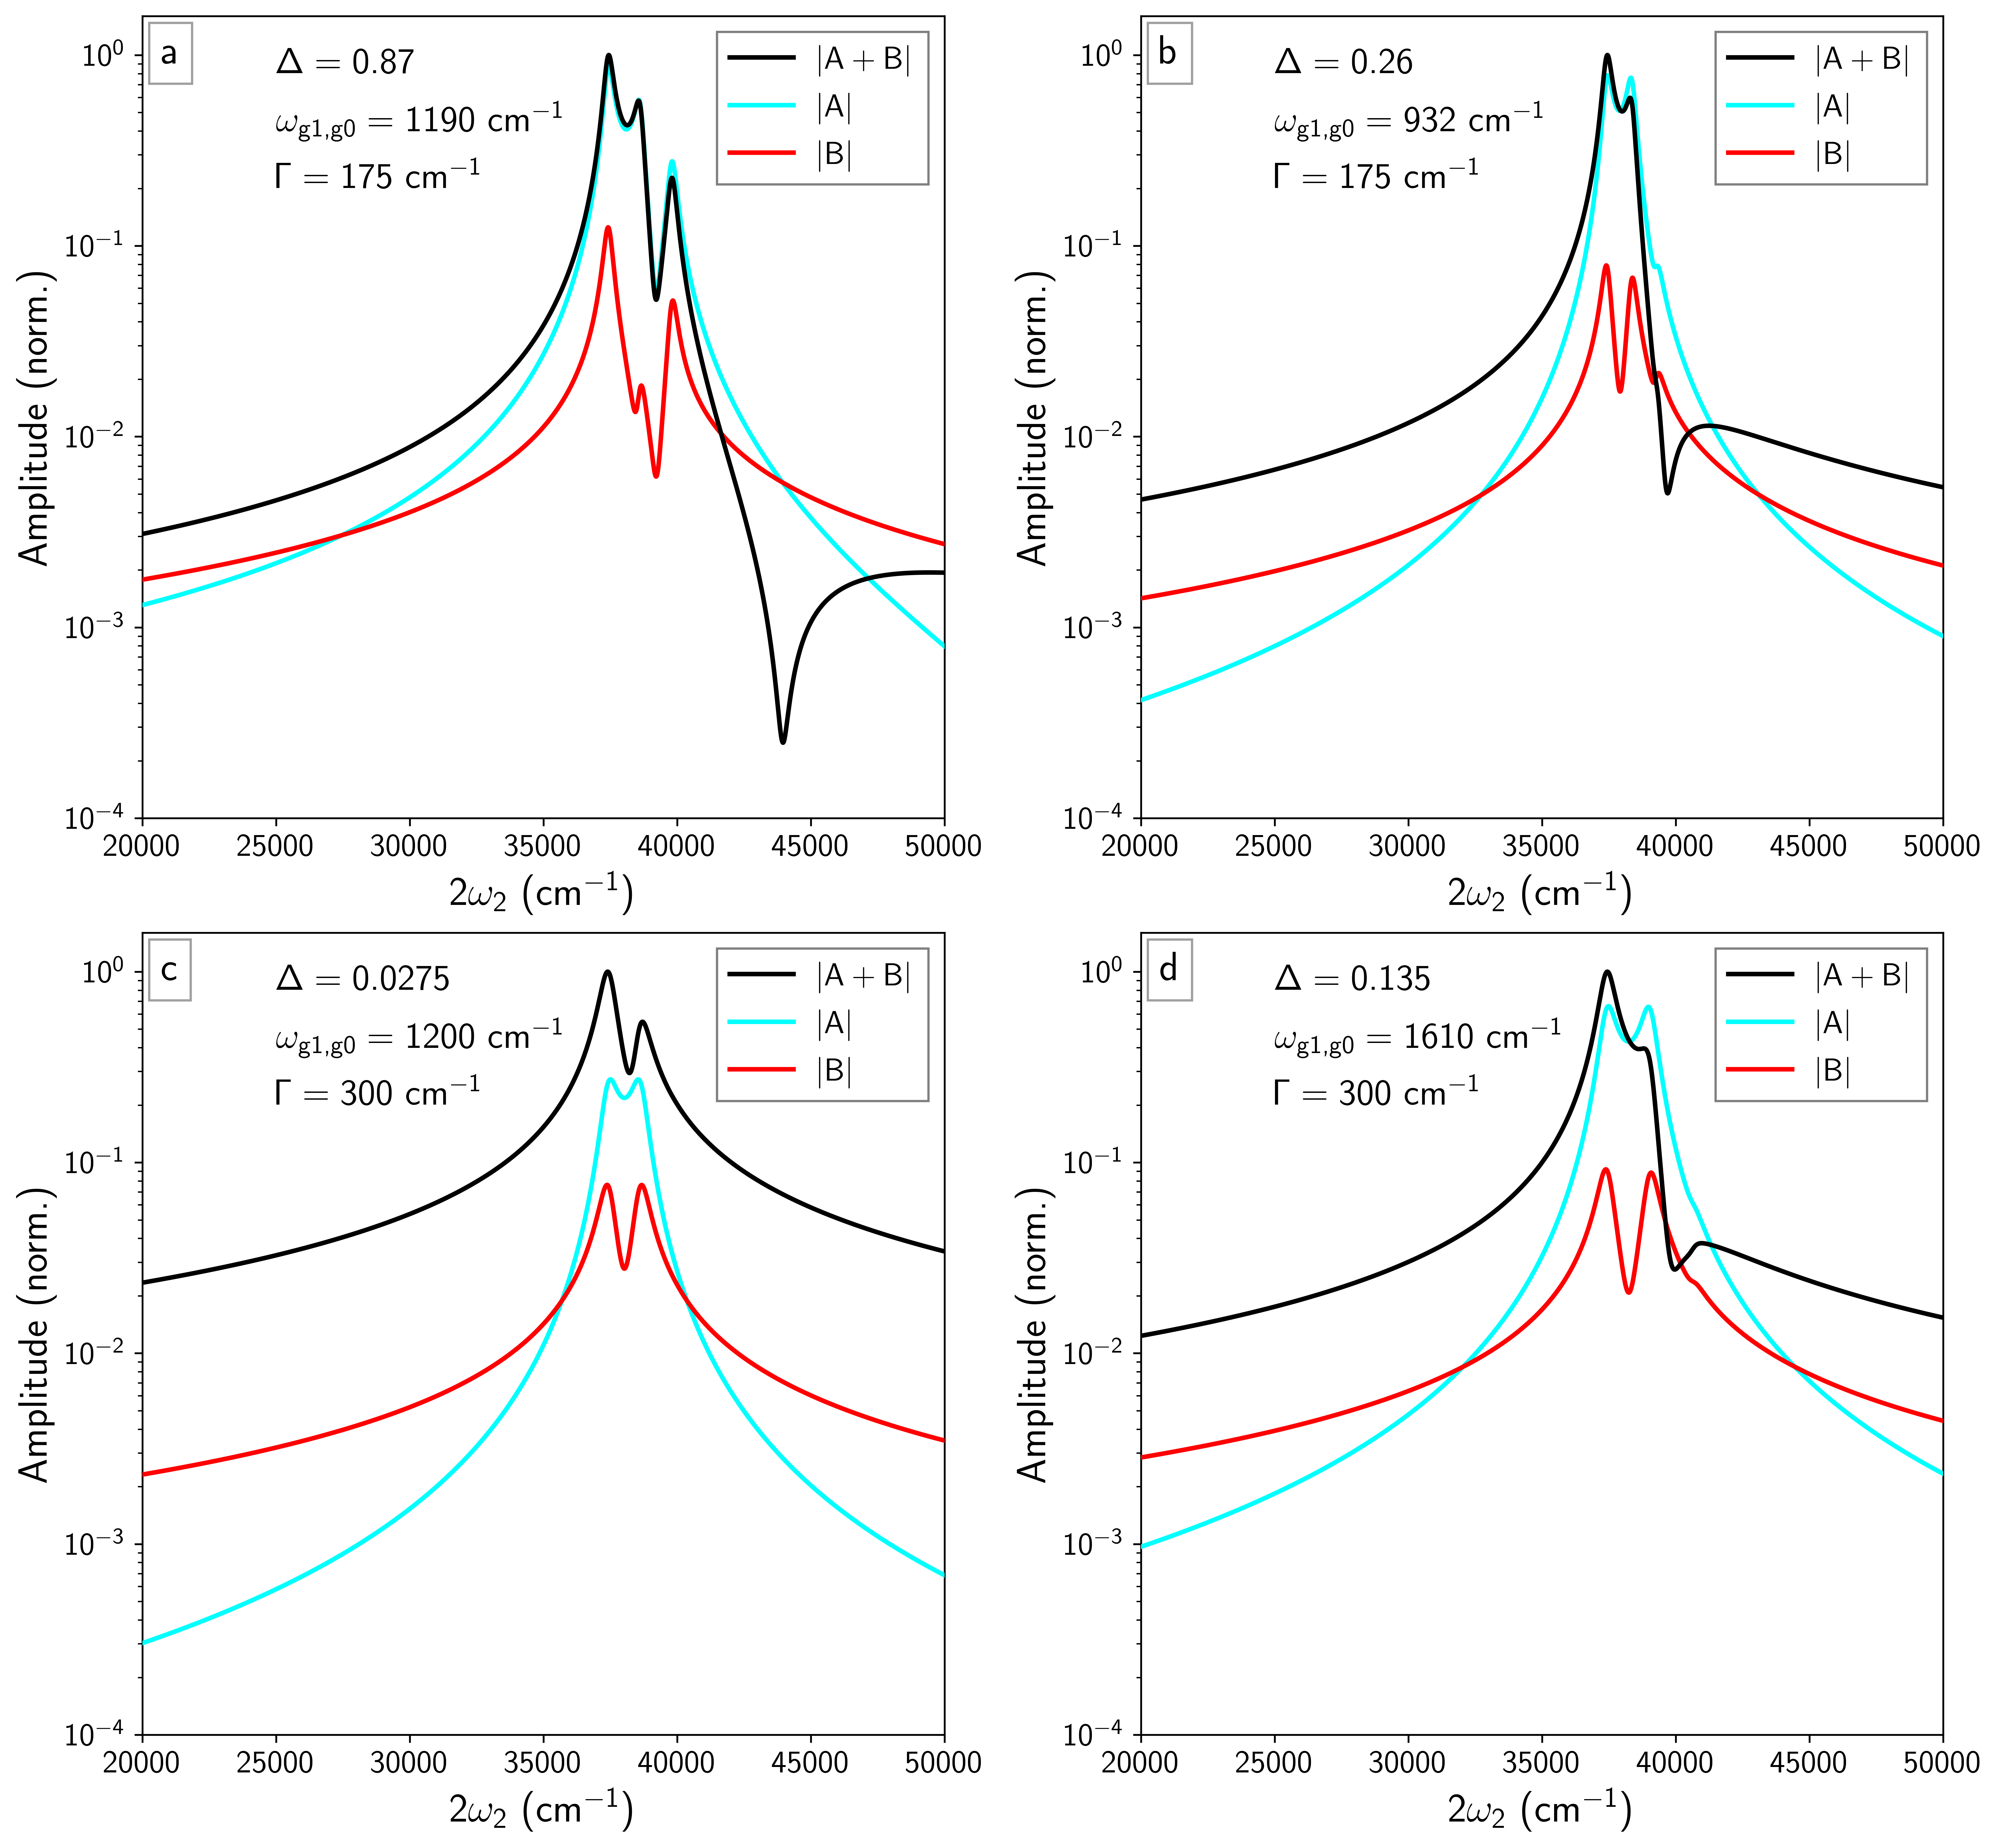
\includegraphics[width=6.675in]{figures/changedelta.png}
	\caption{The impact of offset, vibrational resonance, and linewidth on HDFG spectra. Parameters for (a,b) follow from Myers et al., whereas parameters for (c,d) follow from Brennan et al.\cite{Myers1982, Brennan2024}
	Note that in these plots, the ratio $\abs{A/B} = 0.1$ is enforced.} 
	\label{fig:chgdelta}
\end{figure}

In addition to the linewidth and offset impacting the shape of the HDFG response, the sign of the molecular parameters $M^{ge}_0, \Lambda^{ge}_0, \frac{\partial M^{ge}}{\partial Q} , \frac{\partial \Lambda^{ge}}{\partial Q}$ will significantly impact the HDFG spectrum.
As discussed in the main text, the atypical lineshape in the post-resonance region of the HDFG region arises due to the sign of all four aforementioned parameters being identical.
Changing the sign of one (or three) parameters will change the sign of $A, B$ and eliminate interference between the real and imaginary terms.  
As an example, we demonstrate the resultant HDFG spectrum when $M_0^{ge} < 0$, and all other terms $>0$ (\autoref{fig:chgsign}).
Compared to Figure 3 of the main text, the contributions from the $A, B_1$ and $B_2$ terms to $\Re(\gamma)$ and $\Im(\gamma)$ significantly change.
In particular, $\Re(\gamma)$ and $\Im(\gamma)$ are of similar value in the post-resonance region, eliminating the interference seen in Figure 3 of the main text.

\begin{figure}[!htbp]
	\centering
	\includegraphics[width=6.675in]{figures/drsive_chgsign.png}
	\caption{Contributions of $A, B$ to HDFG spectrum for a simple two harmonic well system, identical to the main text, except $M_0^{ge} < 0$.
		(a) Potential energy surfaces for a two-well system, (b) 1D HDFG spectrum for $\Delta = 0.5$, $\omega_1 = \omega_{g1, g0}$, (c, d) real and imaginary parts of terms plotted in (b), respectively.
		The spectra are referenced to $\max{(A+B)}$. 
		The vibronic one and two photon absorption operators are scaled such that $\abs{B}/\abs{A} \sim$ 0.1, following Chung and Ziegler. \cite{Ziegler1988}
} 
	\label{fig:chgsign}
\end{figure}

\section{Evaluating impact of static inhomogeneity on HDFG output}
In this section, the integral
\begin{equation}\label{generalcontour}
	\begin{split}
		\gamma_{ijkl} &= \int_{-\infty}^\infty \mathrm{d}\xi P(\xi) \gamma_{ijkl}(\xi)\\
		&= \frac{\sigma}{\pi}\int_{-\infty}^\infty \mathrm{d}\xi \frac{1}{\sigma^2 + \xi^2} \frac{\eta_{ijkl}}{\left(\Delta_{ga} - \xi\right)\left(\Delta_{ba}+ c\xi\right)} \\
		&= \frac{\eta_{ijkl} \sigma}{\pi} \int_{-\infty}^\infty \mathrm{d}\xi\frac{1}{(\xi + i\sigma)(\xi - i\sigma)} \frac{1}{\Delta_{ga} - \xi} \frac{1}{\Delta_{ba} + c\xi}\\
	\end{split}
\end{equation}
is evaluated for $c=-1$ (electronic state and vibrational state energy fluctuations are anti-correlated) and $c=1$ (electronic state and vibrational state energy fluctuations are correlated).
Integrals such as those found in \autoref{generalcontour} can be evaluated by using the Residue theorem. %@dan i had too much white space, needed something to fill in... delete if you want.
If a complex valued function $f(z)$ is integrated along a positively oriented closed contour,%guessing on this one
\begin{subequations}\label{eq:generalcontour}
	\begin{equation}
		\oint \mathrm{d}z f(z) = 2\pi i \sum_k \Res[f(z_k)]
	\end{equation}
where the residue of an n$^{\text{th}}$ order pole at $z = z_k$, $\Res[f(z_k)]$ is evaluated as
	\begin{equation}
		\Res[f(z_k)] = \lim_{z \rightarrow z_k} \frac{1}{\left(n-1\right)!} \frac{\mathrm{d}^{n-1}}{\mathrm{d}z^{n-1}} \left[f(z) (z-z_k) \right]
	\end{equation}
For first order poles (the cases considered below), $n=1$, so that 
	\begin{equation}
		\oint \mathrm{d}z f(z) = 2\pi i \sum_k \lim_{z \rightarrow z_k} f(z) (z-z_k)
	\end{equation}
\end{subequations}
Note that in \autoref{eq:generalcontour}, the integrals are closed along a contour which wraps all the poles. 

\subsection{Anti-correlated Modes}
For anti-correlated modes ($c = -1$), the poles ($\xi_k$) are situated in the complex plane as shown in \autoref{fig:contours}a.
Since \autoref{generalcontour} is evaluated along the real axis, one can choose to evaluate the contour in the upper or lower half of the complex plane.
In other words, we can choose the contour which wraps around the least number of poles.
For c = -1, there are four poles: $\pm i \sigma, \Delta_{ga}, \Delta_{ba}$. 
The contour that wraps the upper half of the complex plane has only one pole, $i \sigma$; as such, we choose to evaluate \autoref{generalcontour} in the upper half of the complex plane for the case of anti-correlated modes, as it contains the least number of poles.
Using the residue theorem for a first order pole,\cite{Carlson1990line} we see
\begin{widetext}
	\begin{equation}
		\begin{split}
			\int_{-\infty}^\infty \mathrm{d}\xi P(\xi) \gamma_{ijkl}(\xi) &= 2\pi i \sum_k \lim_{\xi \rightarrow \xi_k} P(\xi) \gamma_{ijkl}(\xi) (\xi - \xi_k)\\
			&= 2\pi i \frac{\eta_{ijkl} \sigma}{\pi} \lim_{\xi \rightarrow i\sigma} \frac{1}{(\xi + i\sigma)(\xi - i\sigma)} \frac{1}{\Delta_{ga} - \xi} \frac{1}{\Delta_{ba} - \xi} (\xi - i \sigma)\\
			&= 2 \eta_{ijkl} \sigma i \lim_{\xi \rightarrow i\sigma} \frac{1}{\xi + i\sigma} \frac{1}{\Delta_{ga} - \xi} \frac{1}{\Delta_{ba} - \xi}\\
			&= 2\eta_{ijkl} \sigma i \frac{1}{2i\sigma} \frac{1}{\Delta_{ga} - i\sigma} \frac{1}{\Delta_{ba} - i\sigma}\\
			&= \frac{\eta_{ijkl}}{\left(\Delta_{ga}-i\sigma\right)\left(\Delta_{ba}-i \sigma\right)}\\
		\end{split}
	\end{equation}
\end{widetext}


\subsection{Correlated Modes}
For correlated modes, the poles are situated in the complex plane as shown in \autoref{fig:contours}b.
It is clear that no matter which contour is chosen, the contour will envelop two poles.
We choose to evaluate along the contour in the bottom half of the complex plane (see \autoref{fig:contours}b), where the poles are $\{-i\sigma, \Delta_{ga}\}$.
Since the $\xi_k$ are nondegenerate,
\begin{widetext}
	\begin{equation}
		\begin{split}
			\int_{-\infty}^\infty \mathrm{d}\xi P(\xi) \gamma_{ijkl}(\xi) &= 2\pi i \sum_k \lim_{\xi \rightarrow \xi_k} P(\xi) \gamma_{ijkl}(\xi) (\xi - \xi_k)\\
			&= 2\pi i \frac{\eta_{ijkl} \sigma}{\pi}  \lim_{\xi \rightarrow -i\sigma} \frac{1}{(\xi + i\sigma)(\xi - i\sigma)} \frac{1}{\Delta_{ga} + \xi} \frac{1}{\Delta_{ba} - \xi} \left(\xi + i \sigma\right) \\ 
			&+ 2\pi i \frac{\eta_{ijkl} \sigma}{\pi} \lim_{\xi \rightarrow \Delta_{ga}} \frac{1}{(\xi + i\sigma)(\xi - i\sigma)} \frac{1}{\Delta_{ga} - \xi} \frac{1}{\Delta_{ba} - \xi} \left(\xi - \Delta_{ga}\right)\\
			&= 2 \eta_{ijkl} i \sigma \left(\frac{1}{2 i \sigma} \frac{1}{-i \sigma - \Delta_{ga}} \frac{1}{\Delta_{ba} - i\sigma} \right) - 2\eta_{ijkl} i \sigma \left(\frac{1}{\sigma^2 + \Delta_{ga} ^2} \frac{1}{\Delta_{ga} + \Delta_{ba}} \right)\\
			&= -\frac{\eta_{ijkl}}{\Delta_{ga} + i \sigma} \left(\frac{1}{\Delta_{ba} - i \sigma} + \frac{2i\sigma}{(\Delta_{ga} - i \sigma)(\Delta_{ga} + \Delta_{ba})}\right)\\
		\end{split}
	\end{equation}
\end{widetext}


\begin{figure}[!htbp]
	\centering
	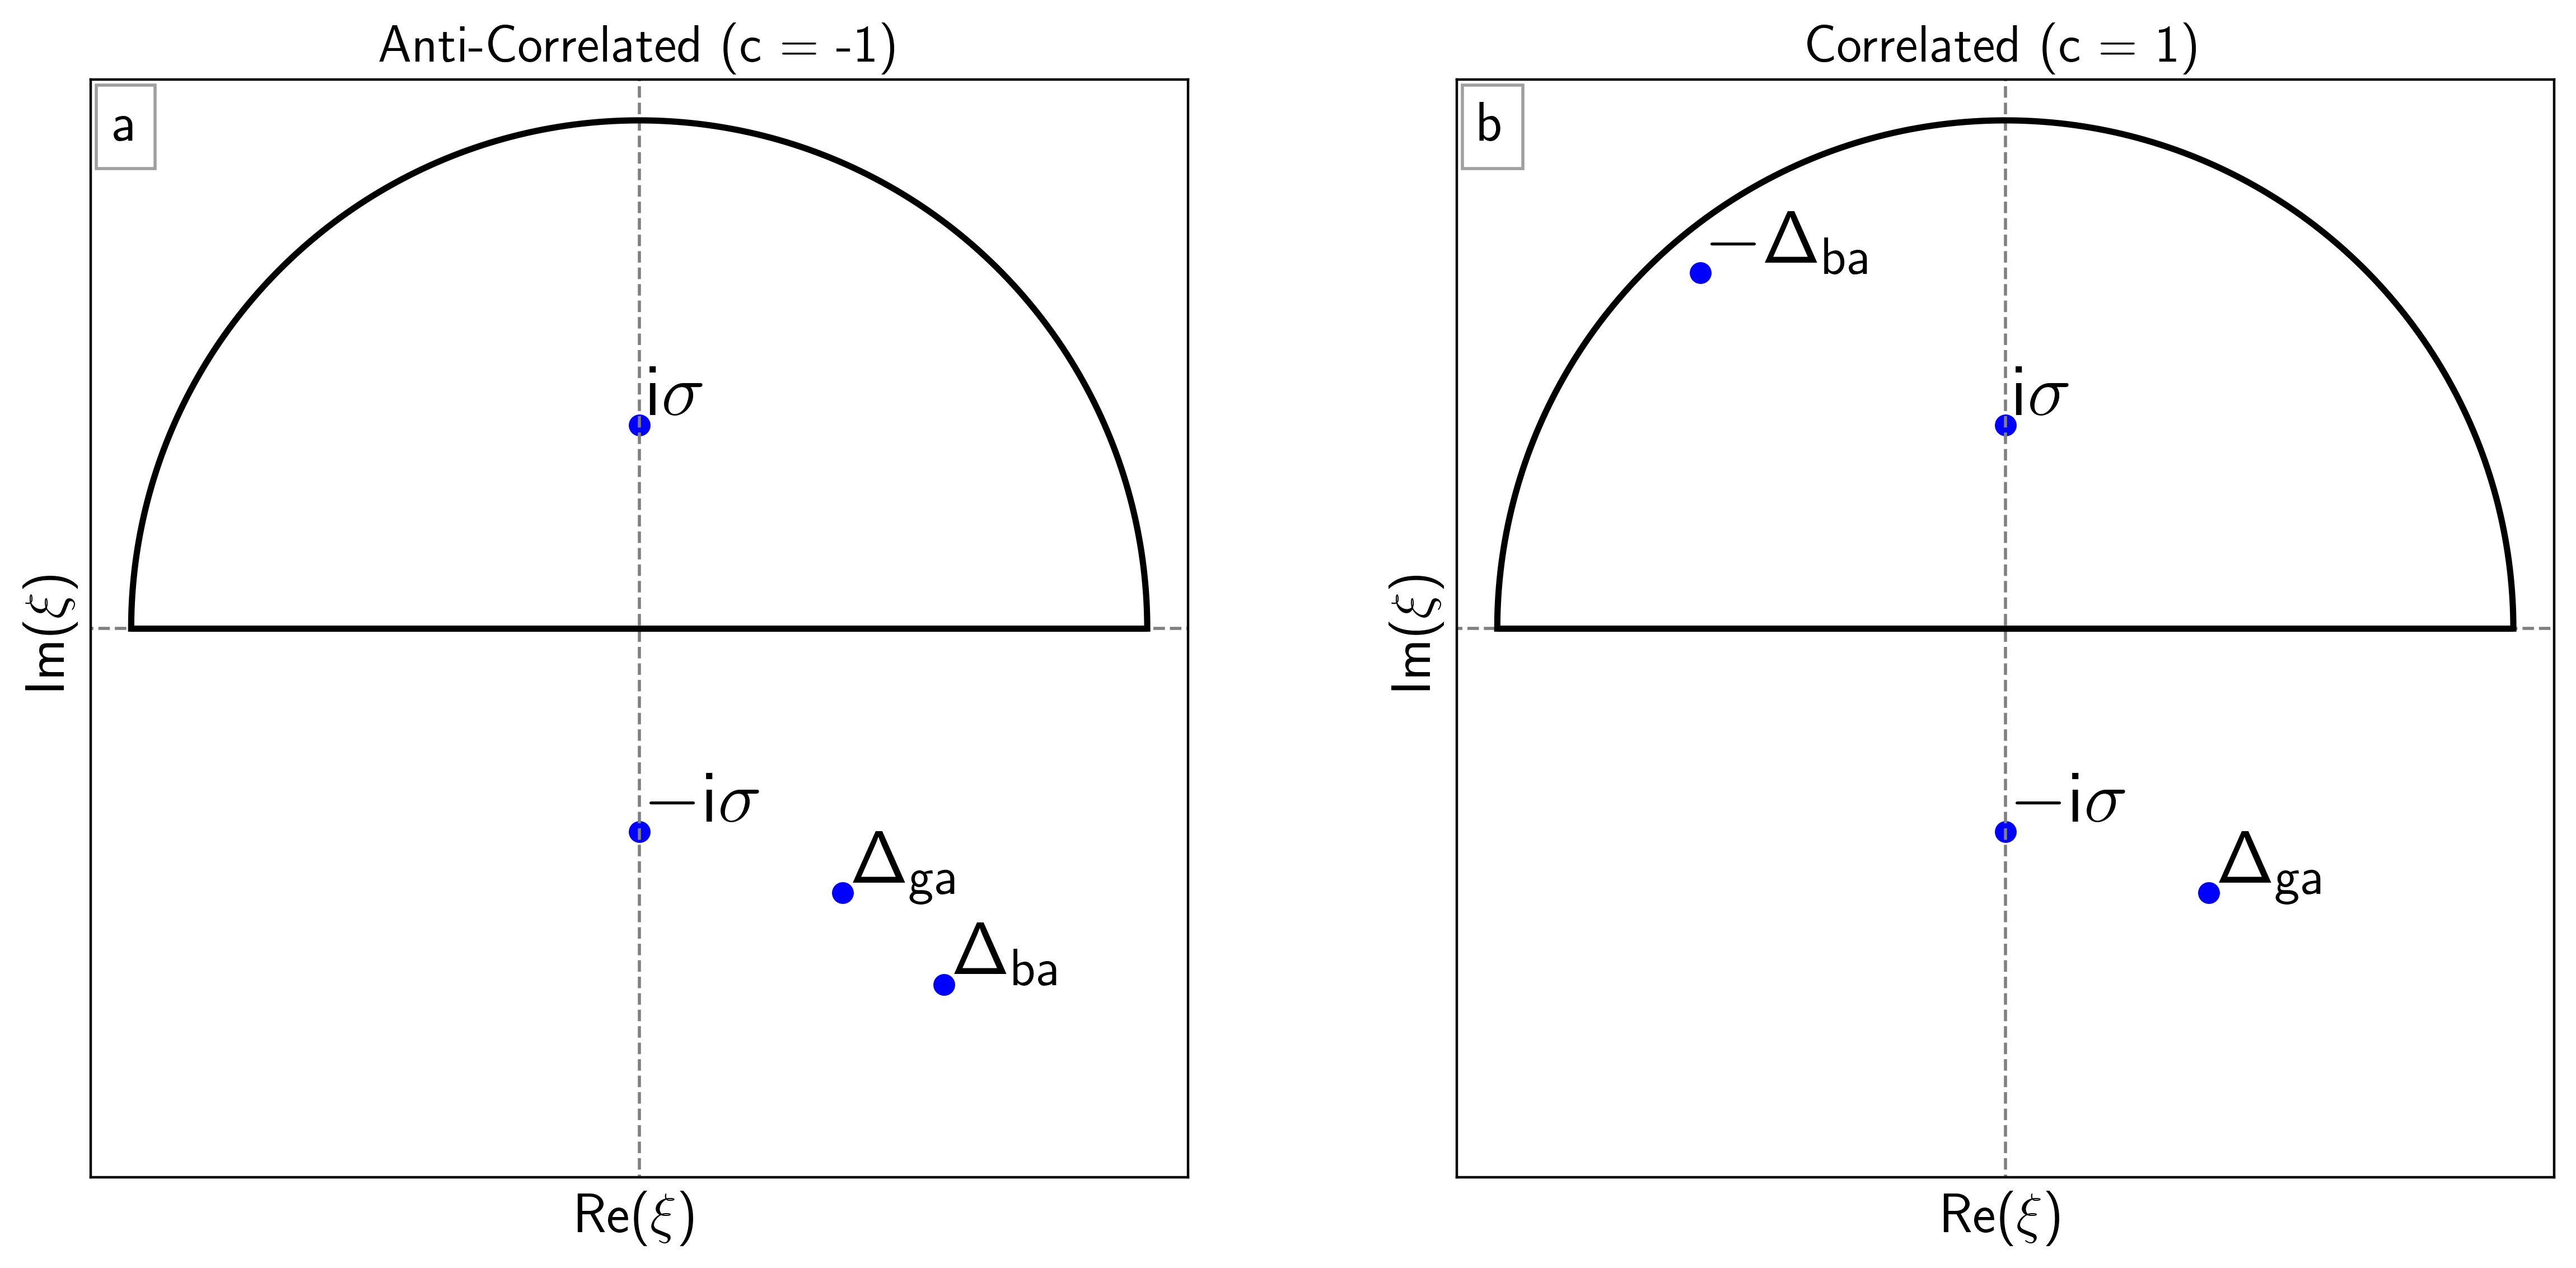
\includegraphics[width=6.675in]{figures/corr_contour.png}
	\caption{Poles (blue dots) and contours (black lines) used to evaluate \autoref{generalcontour} for (a) anti-correlated ($c=-1$) and (b) correlated ($c=1$) modes. 
	} 
	\label{fig:contours}
\end{figure}
\break

\section{References}
% Create the reference section using BibTeX:
\bibliography{library.bib}

\end{document}
%


